\documentclass[12pt]{report}

% Packages
% ========
\usepackage[letterpaper, portrait, margin=1in]{geometry}
\usepackage{graphicx}			% So we can load figures with "." in their filename
\usepackage{float}				% So we can use "[H]"
\usepackage[dvipsnames]{xcolor}	% For custom colors
\usepackage{xparse}				% For \DeclareDocumentCommand
\usepackage{caption}			% For \captionof command
\usepackage{mathtools}			% For \DeclarePairedDelimeter
\usepackage{ifthen}				% For \ifthenelse{}{}{}
\usepackage{soul}				% For underlining with \ul
\setuldepth{x}					%	""
\usepackage{multicol}			% For multiple columns via \begin{multicols}{2}
\usepackage[most]{tcolorbox}	% For the tl; dr environment
\usepackage{array}				% For extended column definitions
\usepackage{tabularray}			% For \begin{longtblr} tables that span multiple columns and pages
\usepackage{amssymb}			% For $\checkmark$
\usepackage{etoc}				% For \localtableofcontents


% Inserting code into LaTeX: \begin{lstlisting} ...
\usepackage{listings}
\definecolor{dkgreen}{rgb}{0,0.6,0}
\definecolor{gray}{rgb}{0.5,0.5,0.5}
\definecolor{mauve}{rgb}{0.58,0,0.82}

\lstset{frame=tb,
  language=C++,
  aboveskip=3mm,
  belowskip=3mm,
  showstringspaces=false,
  columns=flexible,
  basicstyle={\small\ttfamily},
  numbers=none,
  numberstyle=\tiny\color{gray},
  keywordstyle=\color{blue},
  commentstyle=\color{dkgreen},
  stringstyle=\color{mauve},
  breaklines=true,
  breakatwhitespace=true,
  tabsize=3
}

% Inline code
\definecolor{darkpink}{rgb}{0.5, 0.0, 0.5}
\newcommand{\code}[1]{\texttt{\color{darkpink}#1}}

% Bibliography
% ============
\usepackage[american]{babel}
\usepackage{csquotes}
\usepackage[style=ieee, backend=biber]{biblatex}
\usepackage{hyperref}
\hypersetup{colorlinks=true, allcolors=black, urlcolor=blue}
\addbibresource{../sources.bib}

% etoc setup
% ==========

\etocsetstyle{section}{}{}{\etocsavedchaptertocline{\numberline{}\etocname}{\etocpage}}{}
\etocsetstyle{subsection}{}{}{\etocsavedsectiontocline{\numberline{}\etocname}{\etocpage}}{}
\etocsetstyle{subsubsection}{}{}{\etocsavedsubsectiontocline{\numberline{}\etocname}{\etocpage}}{}
\etocsetstyle{paragraph}{}{}{\etocsavedsubsubsectiontocline{\numberline{}\etocname}{\etocpage}}{}
\etocsetstyle{subparagraph}{}{}{\etocsavedparagraphtocline{\numberline{}\etocname}{\etocpage}}{}


% Simple custom commands
% ======================
\makeatletter
\def\maxwidth#1{\ifdim\Gin@nat@width>#1 #1\else\Gin@nat@width\fi} 
\makeatother

\def\todo#1{\selectfont{\color{red}\texttt{\textbf{TODO:} #1}}}

% Sections 'n' such
% =================

\definecolor{chaptColor}{RGB}{0, 83, 161}

\def\chapt#1{
%
	% Default chapter behavior
	\begingroup\color{chaptColor}
	\chapter{#1}
	\endgroup
	
	% Label
	\label{chp:#1}
}

\definecolor{sectColor}{rgb}{0, 0.5, 0.0}
\def\sect#1{\textcolor{sectColor}{\section{#1}}}

\definecolor{subsectColor}{rgb}{0, 0.5, 0.5}
\def\subsect#1{\textcolor{subsectColor}{\subsection{#1}}\noindent}

\definecolor{subsubsectColor}{rgb}{0.747, 0.458, 0}
\def\subsubsect#1{\textcolor{subsubsectColor}{\subsubsection{#1}}}

% TL; DR section
% ==============
\newenvironment{tldr}{\begin{tcolorbox}[colback=gray!20!white,colframe=blue!75!black,title=TL; DR]}{\end{tcolorbox}\vspace*{12pt}}

% Custom math commands
% ====================
\DeclarePairedDelimiter\ceil{\lceil}{\rceil}
\DeclarePairedDelimiter\floor{\lfloor}{\rfloor}

% ======================
% \graphic{filename=...}
% ======================
% Keyword arguments
\makeatletter
\define@key{graphicKeys}{filename}{\def\graphic@filename{#1}}
\define@key{graphicKeys}{scale}{\def\graphic@scale{#1}}
\define@key{graphicKeys}{width}{\def\graphic@width{#1}}
\define@key{graphicKeys}{caption}{\def\graphic@caption{#1}}
\define@key{graphicKeys}{captionType}{\def\graphic@captionType{#1}}
\define@key{graphicKeys}{label}{\def\graphic@label{#1}}

% Kwargs
\DeclareDocumentCommand{\graphic}{m}{

	\begingroup
	
	% Set default kwargs
	\setkeys{graphicKeys}{filename={0}, #1}
	\setkeys{graphicKeys}{scale={0}, #1}
	\setkeys{graphicKeys}{width={0}, #1}
	\setkeys{graphicKeys}{caption={}, #1}
	\setkeys{graphicKeys}{captionType={figure}, #1}
	\setkeys{graphicKeys}{label={}, #1}
	
	% Assign width
	\let\graphicWidth\relax % let \mytmplen to \relax
	\newlength{\graphicWidth}
	\setlength{\graphicWidth}{\columnwidth}
	
	\if \graphic@scale 0
		
		\if \graphic@width 0
			
			\setlength{\graphicWidth}{0.5\columnwidth}
		
		\else
	
			\setlength{\graphicWidth}{\graphic@width}
			
		\fi

	\else
		
		\setlength{\graphicWidth}{\columnwidth * \graphic@scale}

	\fi	
	
	% Do figure
	\begin{minipage}{\columnwidth}
		\vspace*{12pt}
		\begin{center}
		
			\includegraphics[width = \graphicWidth]{\graphic@filename}
			
			\ifthenelse{\equal{\graphic@caption}{}}{}{
				\captionof{\graphic@captionType}{\graphic@caption}
			}
			
			\ifthenelse{\equal{\graphic@label}{}}{
				\label{fig: \graphic@filename}
			}{
				\label{\graphic@label}
			}
		\end{center}
		\vspace*{12pt}
	\end{minipage}
	
	\endgroup
}
\makeatother

% ==============
% Base Pair Page
% ==============
% Keyword arguments
\makeatletter
\define@key{bpPageKeys}{baseFilename}{\def\bpPage@baseFilename{#1}}
\define@key{bpPageKeys}{scale}{\def\bpPage@scale{#1}}
\define@key{bpPageKeys}{width}{\def\bpPage@width{#1}}
\define@key{bpPageKeys}{caption}{\def\bpPage@caption{#1}}
\define@key{bpPageKeys}{captionType}{\def\bpPage@captionType{#1}}
\define@key{bpPageKeys}{label}{\def\bpPage@label{#1}}

% Kwargs
\DeclareDocumentCommand{\BPPage}{m}{

	\begingroup
	
	% Set default kwargs
	\setkeys{bpPageKeys}{baseFilename={0}, #1}
	\setkeys{bpPageKeys}{caption={}, #1}
	\setkeys{bpPageKeys}{label={}, #1}
	
	\newpage

	\begin{center}
		\ul{\mbox{\bpPage@baseFilename{}: 1 Base Pair [min]}}
	\end{center}
	\vspace*{-36pt}
	\begin{minipage}[b]{0.5\textwidth}
		\graphic{filename=\bpPage@baseFilename-overview-1-table, width=\textwidth}
	\end{minipage}
	\begin{minipage}[b]{0.5\textwidth}
		\graphic{filename=\bpPage@baseFilename-overview-1-plot, width=\textwidth}
	\end{minipage}

	\begin{center}
		\ul{\mbox{\bpPage@baseFilename{}: 50 Base Pairs [average]}}
	\end{center}
	\vspace*{-36pt}
	\begin{minipage}[b]{0.5\textwidth}
		\graphic{filename=\bpPage@baseFilename-overview-50-table, width=\textwidth}
	\end{minipage}
	\begin{minipage}[b]{0.5\textwidth}
		\graphic{filename=\bpPage@baseFilename-overview-50-plot, width=\textwidth}
	\end{minipage}
	
	\begin{center}
		\ul{\mbox{\bpPage@baseFilename{}: 100 Base Pairs [max]}}
	\end{center}
	\vspace*{-36pt}
	\begin{minipage}[b]{0.5\textwidth}
		\graphic{filename=\bpPage@baseFilename-overview-100-table, width=\textwidth}
	\end{minipage}
	\begin{minipage}[b]{0.5\textwidth}
		\graphic{filename=\bpPage@baseFilename-overview-100-plot, width=\textwidth}
	\end{minipage}

	\vspace*{-24pt}
	\captionof{figure}{\bpPage@caption}\label{\bpPage@label}	
	
	\endgroup
}
\makeatother



\begin{document}

\textbf{\color{red}Last updated: 2022/07/04 kkona}

\begin{tldr}
	\begin{itemize}
		\item{Some types have an immunity, but Electric is healed by other Electric Types instead of damaged}
		\item{Attacking:
			\begin{itemize}
				\item{``Best'' attackers:
					\begin{itemize}
						\item{Fire}
						\item{Electric}
						\item{Ice}
						\item{Earth}
						\item{Void}
					\end{itemize}
				}
				\item{``Worst'' attackers:
					\begin{itemize}
						\item{Toxic}
						\item{Sound}
						\item{Nature}
						\item{Fire}
					\end{itemize}
				}
			\end{itemize}
			}
		\item{Defending:
			\begin{itemize}
				\item{``Best'' defenders:
					\begin{itemize}
						\item{Metal}
						\item{Earth}
						\item{Void}
						\item{Water}
					\end{itemize}
				}
				\item{``Worst'' defenders:
					\begin{itemize}
						\item{Air}
						\item{Nature}
						\item{Water}
						\item{Metal}
					\end{itemize}
				}
			\end{itemize}
		}
	\end{itemize}
	Note: Types may be found, analyzed, and modified using an EditorUtilityWidget found under \texttt{Content/Editor/Type-Advantage}, right-clicking the \texttt{TypeAdvantages} widget, and selecting \texttt{Run Editor Utility Widget}.
\end{tldr}

\newpage

\sect{Map from Pok\'{e}mon}

\begin{figure}[H]
\begin{center}
	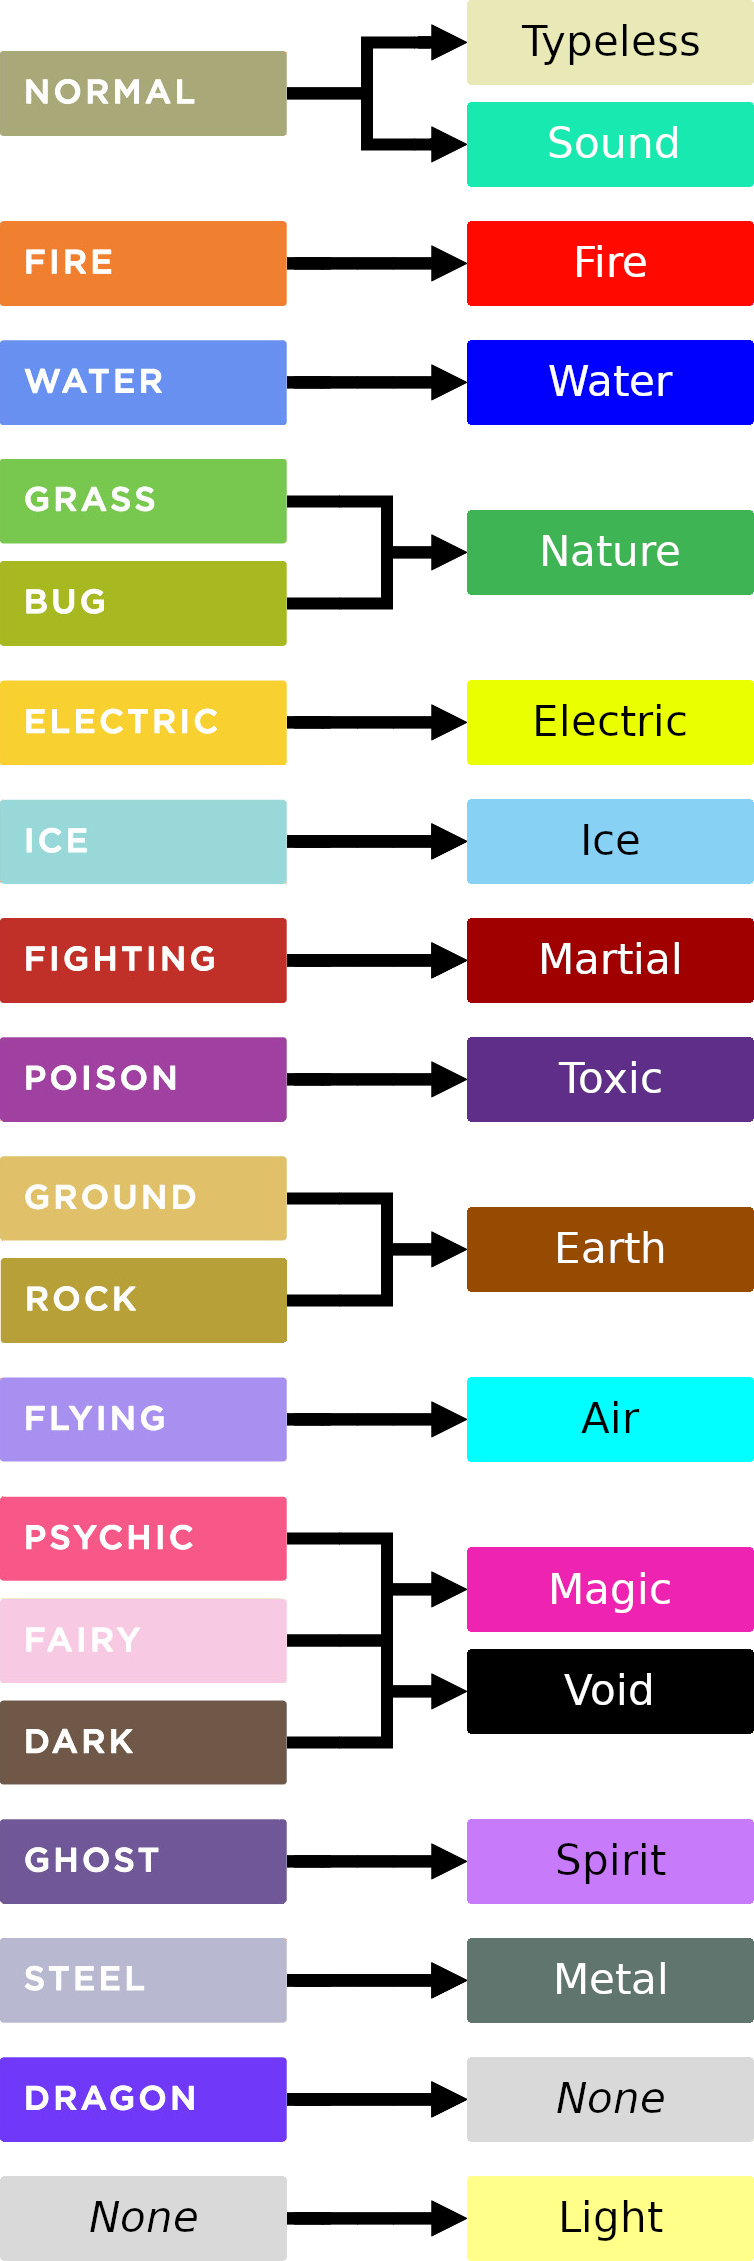
\includegraphics[scale=0.8]{map-from-pkmn}
	\caption{The 18 Pok\'{e}mon types (left) approximately mapped to the 16 Gene Hunter Types (right).}
\end{center}
\end{figure}


\newpage

\sect{Data}
The raw data acquired from the statistics tab of the type advantages UI (see Figure~\ref{fig:stats-ui}) can be found under the ``Type-Matchup-Statistics-Copy'' folder. They're formatted as .tex tables in case I ever wanted to print them, but they can be opened up with any text editor (think Notepad). As pictured, Typeless has been excluded in the analysis.gith

I don't recommend parsing through it unless you're looking for something specific. For example, the 2v2 data has 126 entries. The full data is always available by running the UI as seen in the figure below.

\begin{figure}[H]
	\begin{center}
		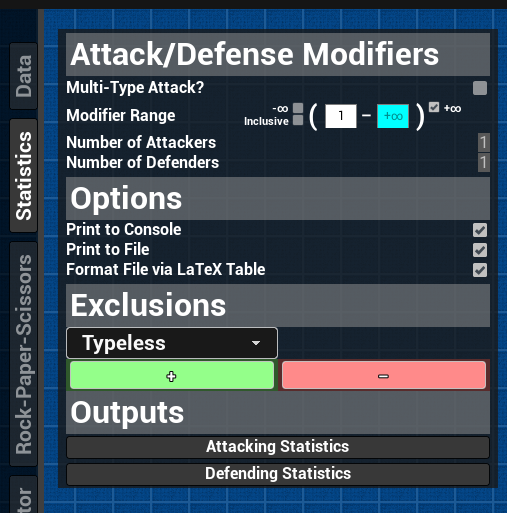
\includegraphics[scale=2]{statistics-ui}
		\caption{The statistics UI (from which the data was acquired).}
		\label{fig:stats-ui}
	\end{center}
\end{figure}

The following sub-sections list data. The Type numbers in parentheses are the sum of advantages\footnote{or resists, or disadvantages, or whatever.} of single- and dual-Type defenders. For example, in the first sub-section, Fire has 4 single advantages and 68 dual advantages for a total of 72 Types.

A minimum of five Types are listed, or more when there is a tie for fifth place.


\subsect{Attacking}
When attacking, ``best'' is defined as most effective and ``worst'' is defined as the most resisted. In practice, these may not so easily be defined.



\subsubsect{Best Single-Type Attackers}

\begin{itemize}
	\item{Fire (72)}
	\item{Electric (69)}
	\item{Ice (69)}
	\item{Earth (63)}
	\item{Void (63)}
\end{itemize}

\subsubsect{Best Dual-Type Attackers}

\begin{itemize}
	\item{Earth + Ice (132)}
	\item{Electric + Void (132)}
	\item{Fire + Nature (129)}
	\item{Earth + Electric (128)}
	\item{Ice + Void (128)}
\end{itemize}

\noindent Note: not surprisingly, these are just combinations of the best single-Type attackers plus Nature.

\subsubsect{Worst Single-Type Attackers}

\begin{itemize}
	\item{Toxic (92)}
	\item{Sound (86)}
	\item{Nature (80)}
	\item{Fire (72)}
	\item{Earth (69)}
	\item{Martial (69)}
\end{itemize}

\subsubsect{Worst Dual-Type Attackers}
\begin{itemize}
	\item{Fire + Sound (53)}
	\item{Fire + Martial (44)}
	\item{Earth + Void (41)}
	\item{Nature + Toxic (35)}
	\item{Earth + Sound (34)}
\end{itemize}

\subsect{Defending}
When defending, ``best'' is defined as most resists and ``worst'' is defined as the most weak to. In practice, these may not so easily be defined.

\subsubsect{Best Single-Type Defenders}
\begin{itemize}
	\item{Earth (16$^*$)}
	\item{Metal (16$^*$)}
	\item{Void (16$^*$)}
	\item{Nature (16)}
	\item{Water (16)}
\end{itemize}
$^*$denotes at least one immunity.

\subsubsect{Best Dual-Type Defenders}
\begin{itemize}
	\item{Electric$^{**}$ + Metal$^*$ (36)}
	\item{Electric$^{**}$ + Void$^*$ (36)}
	\item{Earth$^*$ + Magic (36)}
	\item{Fire + Void$^*$ (36)}
	\item{Ice + Metal$^*$ (36)}
	\item{Magic + Water (36)}
\end{itemize}
$^*$denotes at least one immunity.\\
$^{**}$denotes at least one healed-instead-of-damaged.

\subsubsect{Worst Single-Type Defenders}
\begin{itemize}
	\item{Air (104)}
	\item{Water (104)}
	\item{Metal (104)}
	\item{Nature (104)}
	\item{Fire (81)}
	\item{Void (81)}
	\item{Earth (81)}
\end{itemize}

\subsubsect{Worst Dual-Type Defenders}
\begin{itemize}
	\item{Fire + Metal (144)}
	\item{Void + Water (144)}
	\item{Void + Fire (144)}


	
	\item{Void + Earth (125)}	

	\item{Air + Ice (125)}	
	\item{Air + Magic (125)}
	\item{Air + Martial (125)}
	\item{Air + Nature (125)}
	\item{Air + Spirit (125)}
	\item{Air + Void (125)}
		
	\item{Magic + Water (125)}

	\item{Nature + Ice (125)}
	\item{Nature + Light (125)}
	\item{Nature + Sound (125)}
	\item{Nature + Water (125)}
	\item{Nature + Void (125)}	

	
	\item{Fire + Spirit (125)}

	\item{Metal + Toxic (125)}


\end{itemize}

\newpage

\sect{Type Traits}

As an additional balancing tool, all Types will have traits (including Typeless). This is essential: we do not want to strike balance by doing the analysis as we've done above. For example, can you imagine how boring it would be if every Type had exactly 3~weaknesses and 3~resistances? It would be equally boring to have two or three Types be dominant and the rest to fall into F-tier. Instead each Type should have its own unique identity and balance should not be so black-and-white.\footnote{The old Pok\'{e}mon games promised that I could ``play with the Types I like,'' but that hope was crushed when Bug-types were found to be non-viable in OU (mostly). Scyther was almost saved with Scizor, and even Volcarona fell to UU before long. Why have these scrap types? For the sole purpose of pacing the early game? I found I had to throw away the Beedrill I fell in love with, and so this is my revenge!} Therefore, the following has been proposed:

\begin{longtblr}[
	caption = {Type Trait Suggestions},
	label = {type-traits},
]{
	colspec= {l X[wd=15em]},
	hline{1,Z} = {2pt},
	hlines,
	row{1} = {font=\bfseries},
}

	Type 	& Description\\
	Air 	& Flight lowers the gravity scale and raises the jump height (maybe even flies one day?).\\
	Ice		& Frost armor that regenerates when not taking damage.\\
	Magic	& 5th attack slot for Magic-only utility moves (such as teleportation or cis/transdimensional portal). Magic's dis/advantages are too beige, and this gives the player an incentive to have at least a Magic dual-Type.\\
	Martial	& A c-c-c-combo! meter that fills by damaging within a certain window or by using all moves in a certain order. The reward should be extra damage on the next attack or entering a berserk state. Martial \textit{really} needs something because it's so bland on paper.\\
	Nature	& {Regrowth: HoT that starts when not taking damage and stops when taking damage\\
				\\
				Bark armor that prevents damage on switch for x seconds}\\
	Typeless	& 2x STAB instead of 1.5x (tune as needed!)\\
	
	

\end{longtblr}

These are not complete, as I'm certain future team members will have better ideas than mine. 

\sect{Type Groups}

The Types fit nicely into two or three group schemes. The reason for these groups could be gym-esque leaders, talent tree options, or other game mechanics.

\begin{longtblr}[
	caption = {Type Scheme 1},
	label = {type-scheme-1},
]{
	hline{1,Z} = {2pt},
	hlines,
	row{1} = {font=\bfseries},
}

	Group Name	& Types\\
	Arctic		& {Air\\Ice\\Water}\\
	Desert		& {Earth\\Fire\\Metal}\\
	Energy		& {Electric\\Light\\Sound}\\
	Jungle		& {Martial\\Nature\\Toxic}\\
	Paranormal	& {Magic\\Spirit\\Void}\\

\end{longtblr}

%----------------------------------------

\begin{longtblr}[
	caption = {Type Scheme 2},
	label = {type-scheme-2},
]{
	hline{1,Z} = {2pt},
	hlines,
	row{1} = {font=\bfseries},
}

	Group Name	& Types\\
	Energy		& {Fire\\Light\\Sound}\\
	Jungle		& {Air\\Nature\\Toxic}\\
	Paranormal	& {Magic\\Spirit\\Void}\\
	Planetary	& {Earth\\Ice\\Water}\\
	Power		& {Electric\\Martial\\Metal\\(Typeless?)}\\

\end{longtblr}

%----------------------------------------

\begin{longtblr}[
	caption = {Type Scheme 3},
	label = {type-scheme-3},
]{
	hline{1,Z} = {2pt},
	hlines,
	row{1} = {font=\bfseries},
}

	Group Name	& Types\\
	Arctic		& {Air\\Ice}\\
	Combat		& {Martial\\Metal}\\
	Energy		& {Electric\\Sound}\\
	Island		& {Earth\\Water}\\
	Jungle		& {Nature\\Toxic}\\
	Null		& {Typeless\\Void}\\
	Paranormal	& {Magic\\Spirit}\\
	Solar		& {Fire\\Light}\\

\end{longtblr}

\end{document}